% ===================================
\begin{figure}[t!]
  \centering
  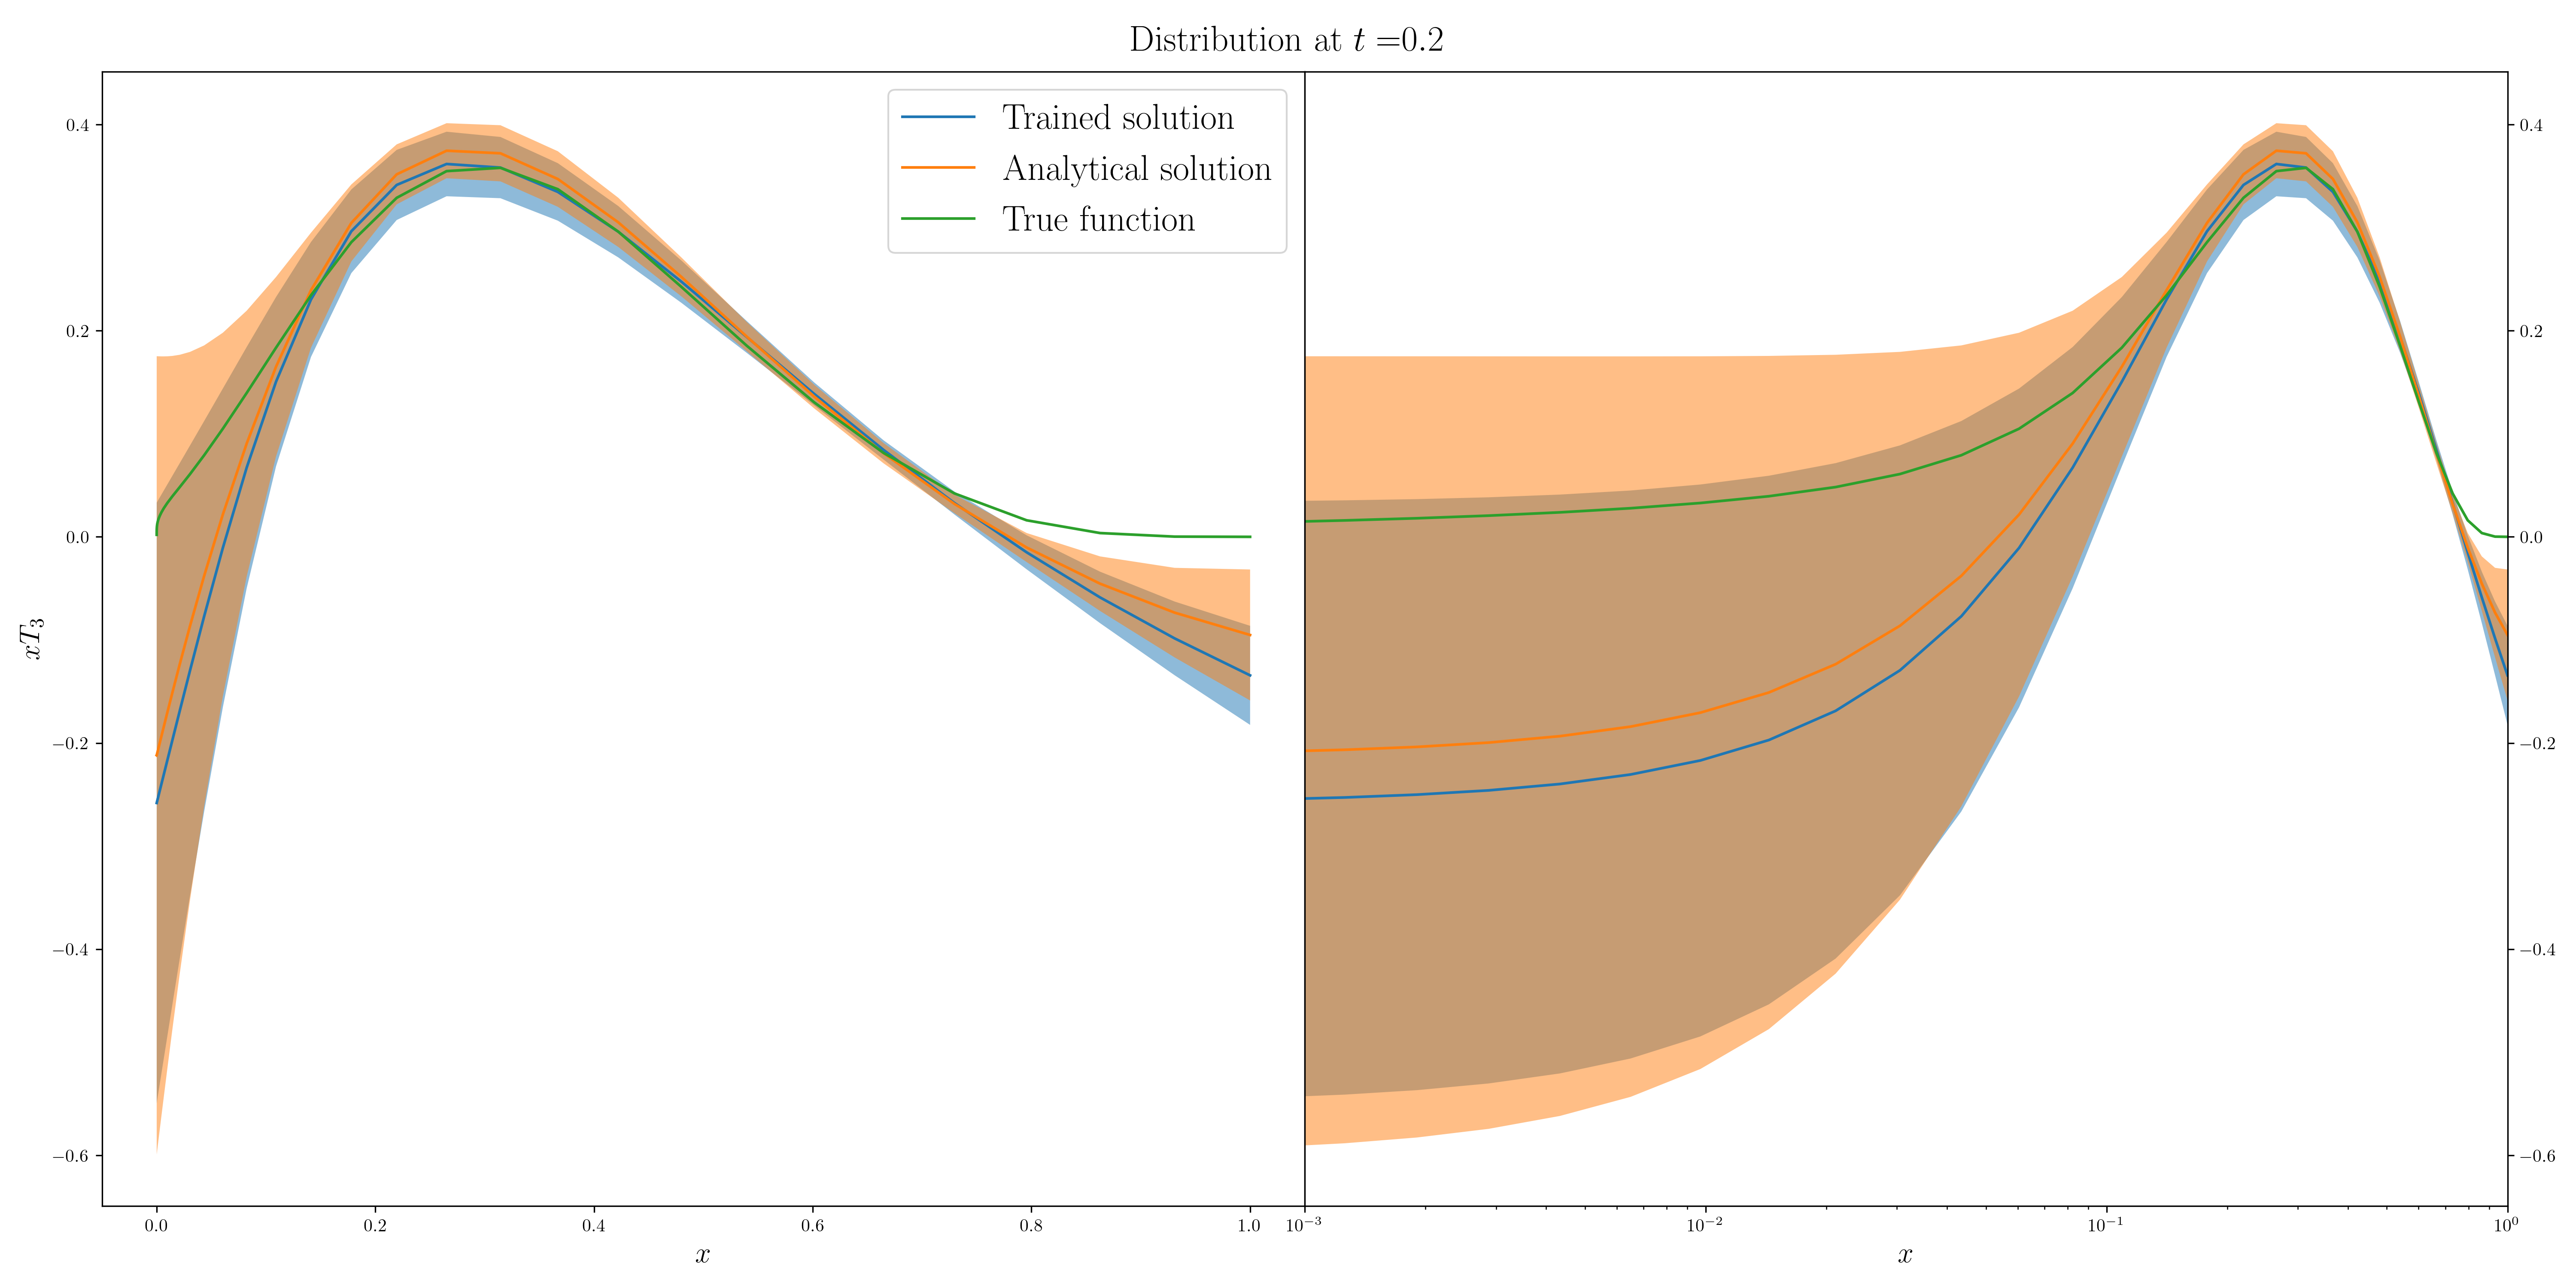
\includegraphics[width=0.65\textwidth]{plots/xT3_2.png}
  \caption{Comparison of the trained solution at the end of training (eot) and analytical solution.
  The boundary condition of the analytical solution is the trained function at $T_{\rm ref} < T_{\rm eot}$,
  and then evolved to $T_{\rm eot}$. The NTK is chosen at $T_{\rm ref}$ too../
  \ac{These plots will be modified (font size, etc...) to match the other figures.}}
  \label{fig:xT3_analytical}
\end{figure}
% ===================================

% ===================================
\begin{figure}[t!]
  \centering
  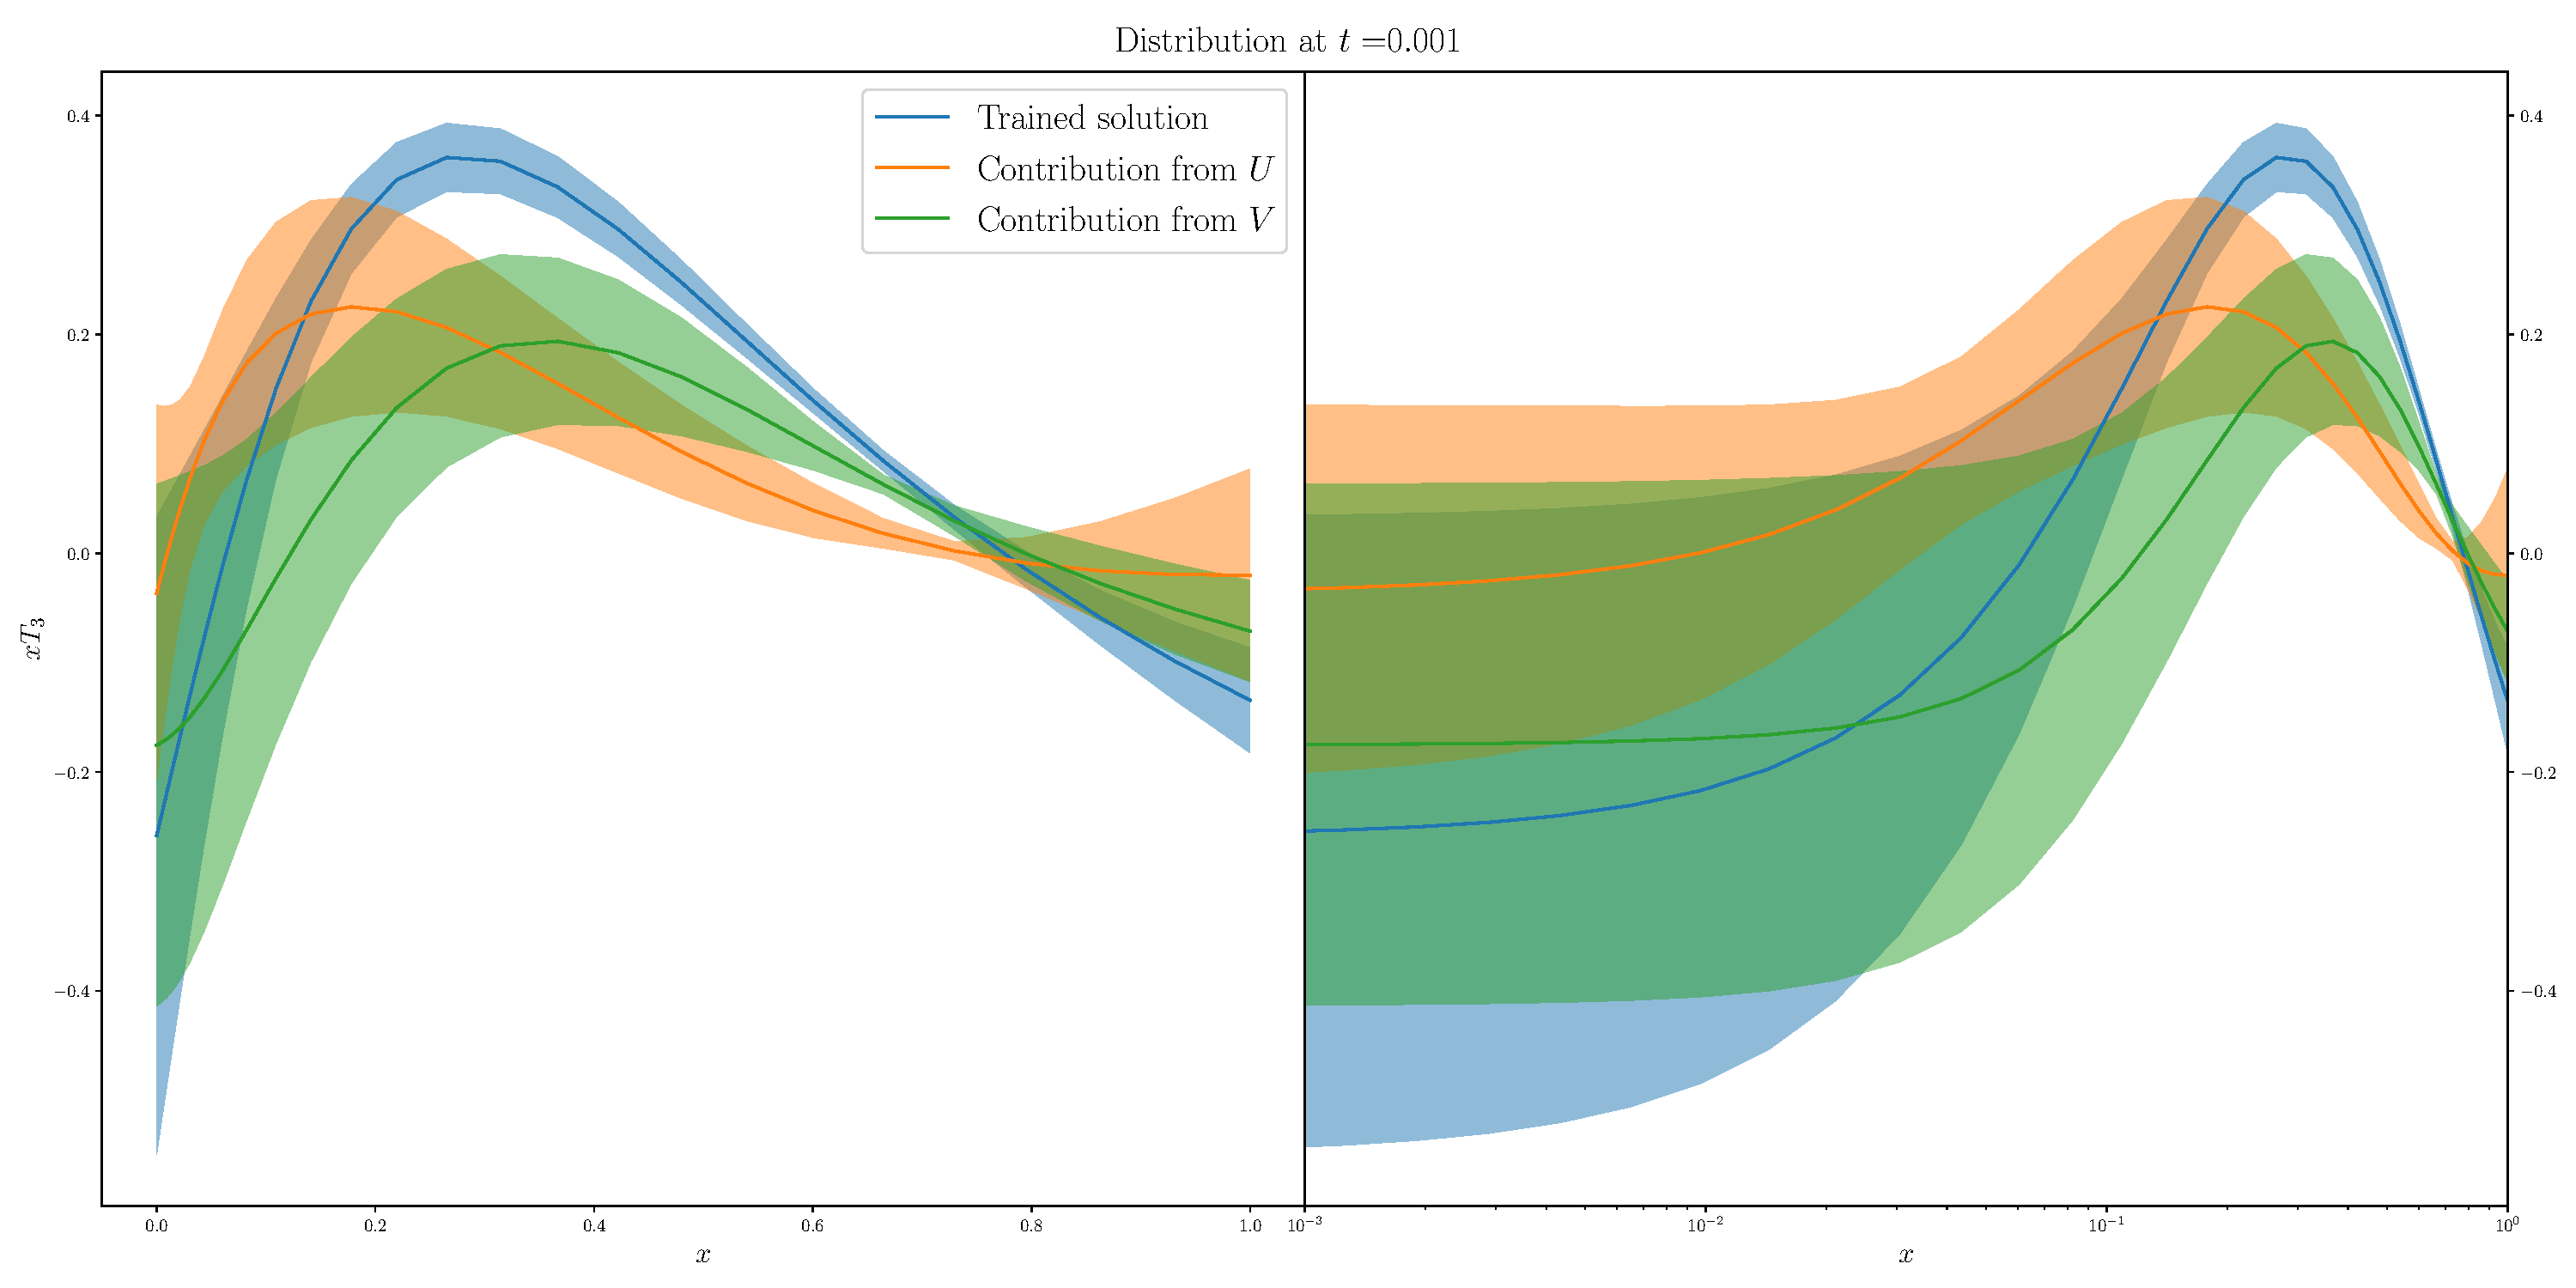
\includegraphics[width=0.65\textwidth]{plots/xT3_u_v_contribution_small_t.pdf} \\
  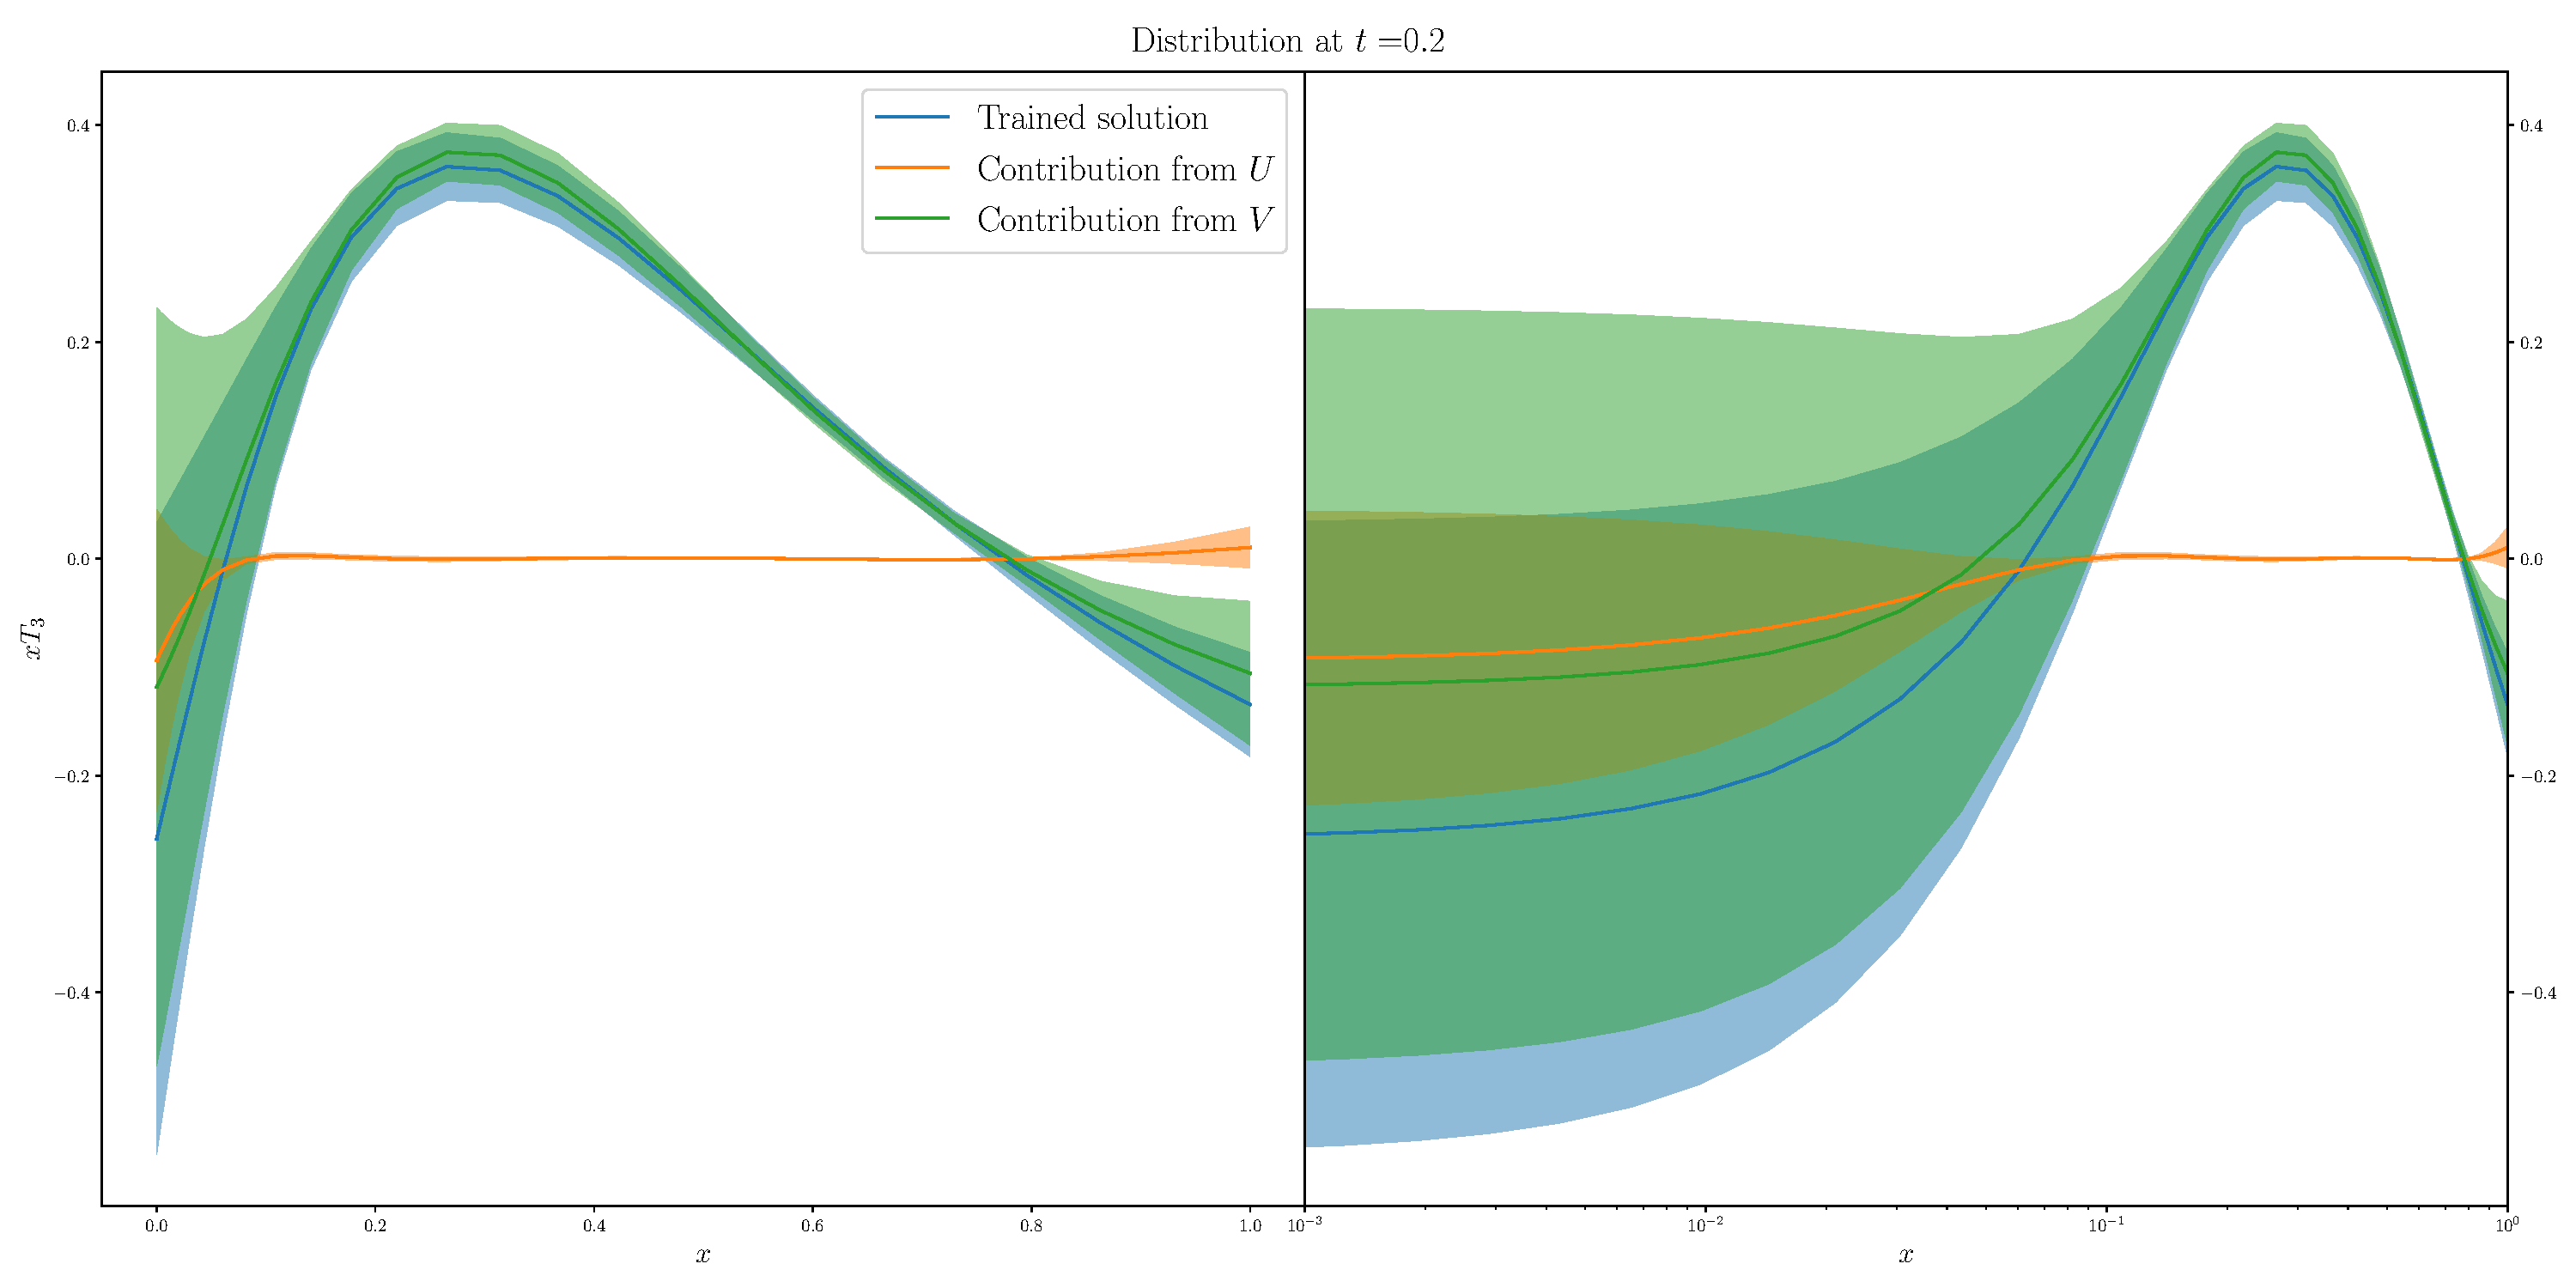
\includegraphics[width=0.65\textwidth]{plots/xT3_u_v_contribution_eot.pdf}
  \caption{Contribution of the $U$ and $V$ terms to the solution. The top panel shows this breakdown
  at early stages of the analytical training ($t=0.001$); the bottom panel shows the contributions at the end
  of training (eot) (same as Fig.~\ref{fig:xT3_analytical}). These plots have been obtained by taking the $t_{\rm ref} = 30000$
  and $f_0 = f_{t_{\rm ref}}$ using L2 data.
  \ac{These plots will be modified (font size, etc...) to match the other figures.}}
\end{figure}
% ===================================

\begin{figure}[t!]
  \centering
  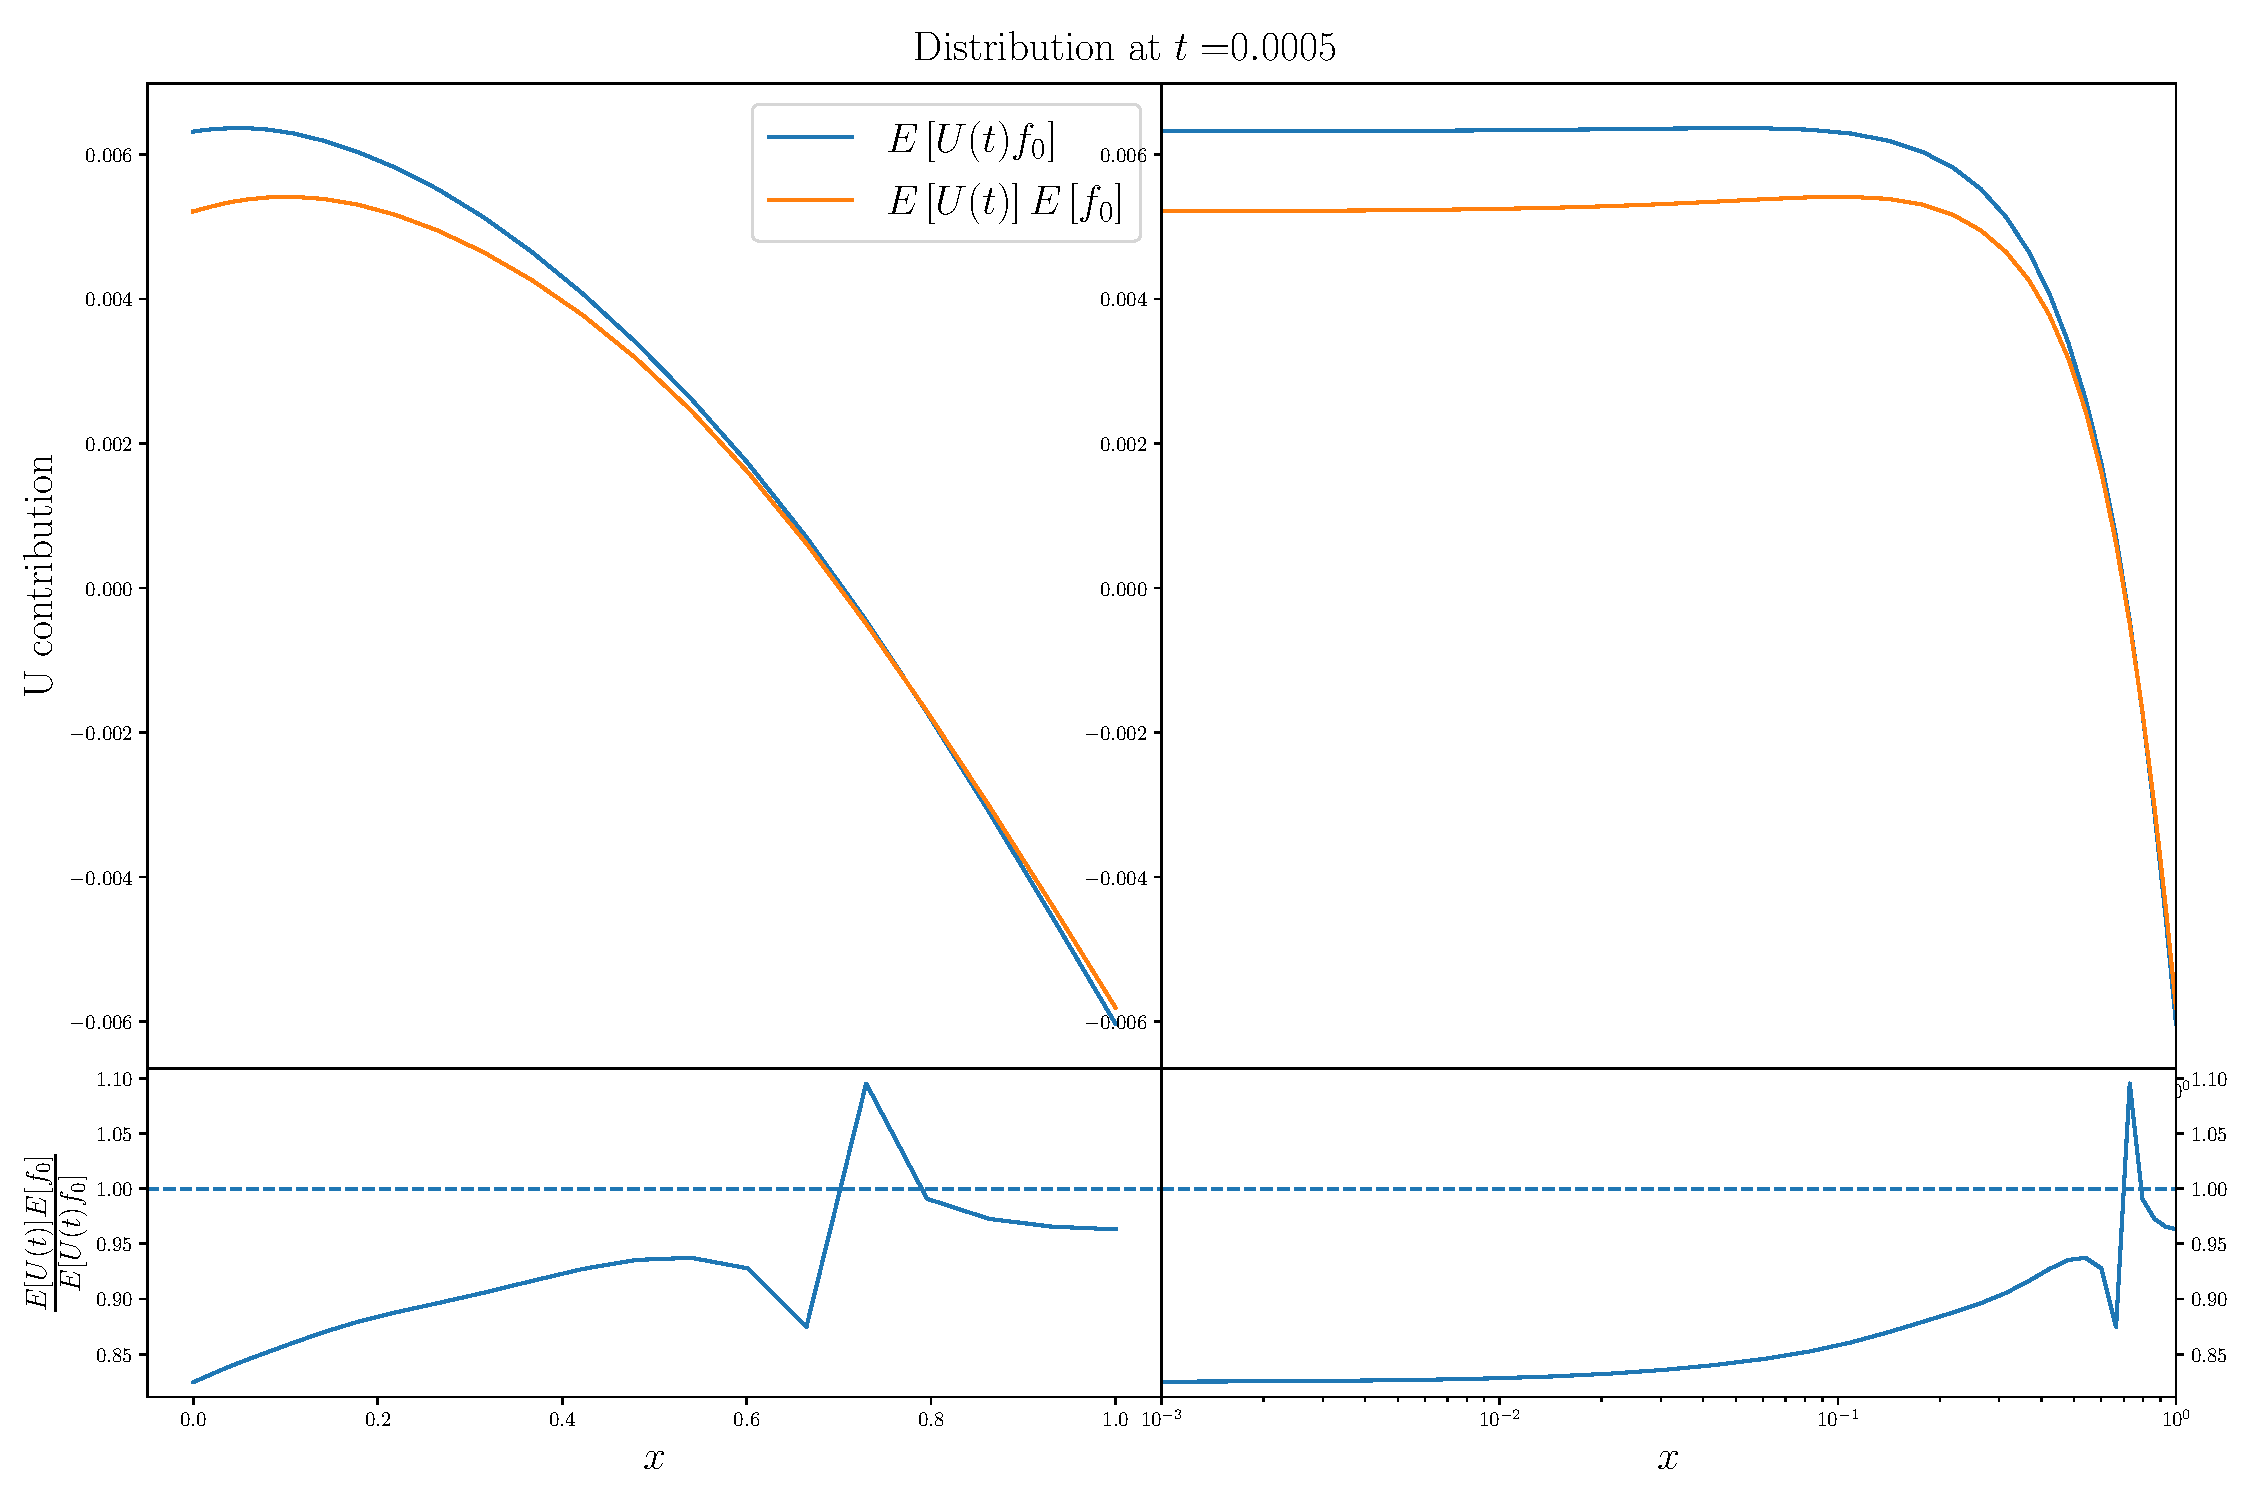
\includegraphics[width=0.65\textwidth]{plots/xT3_exp_val_early.pdf} \\
  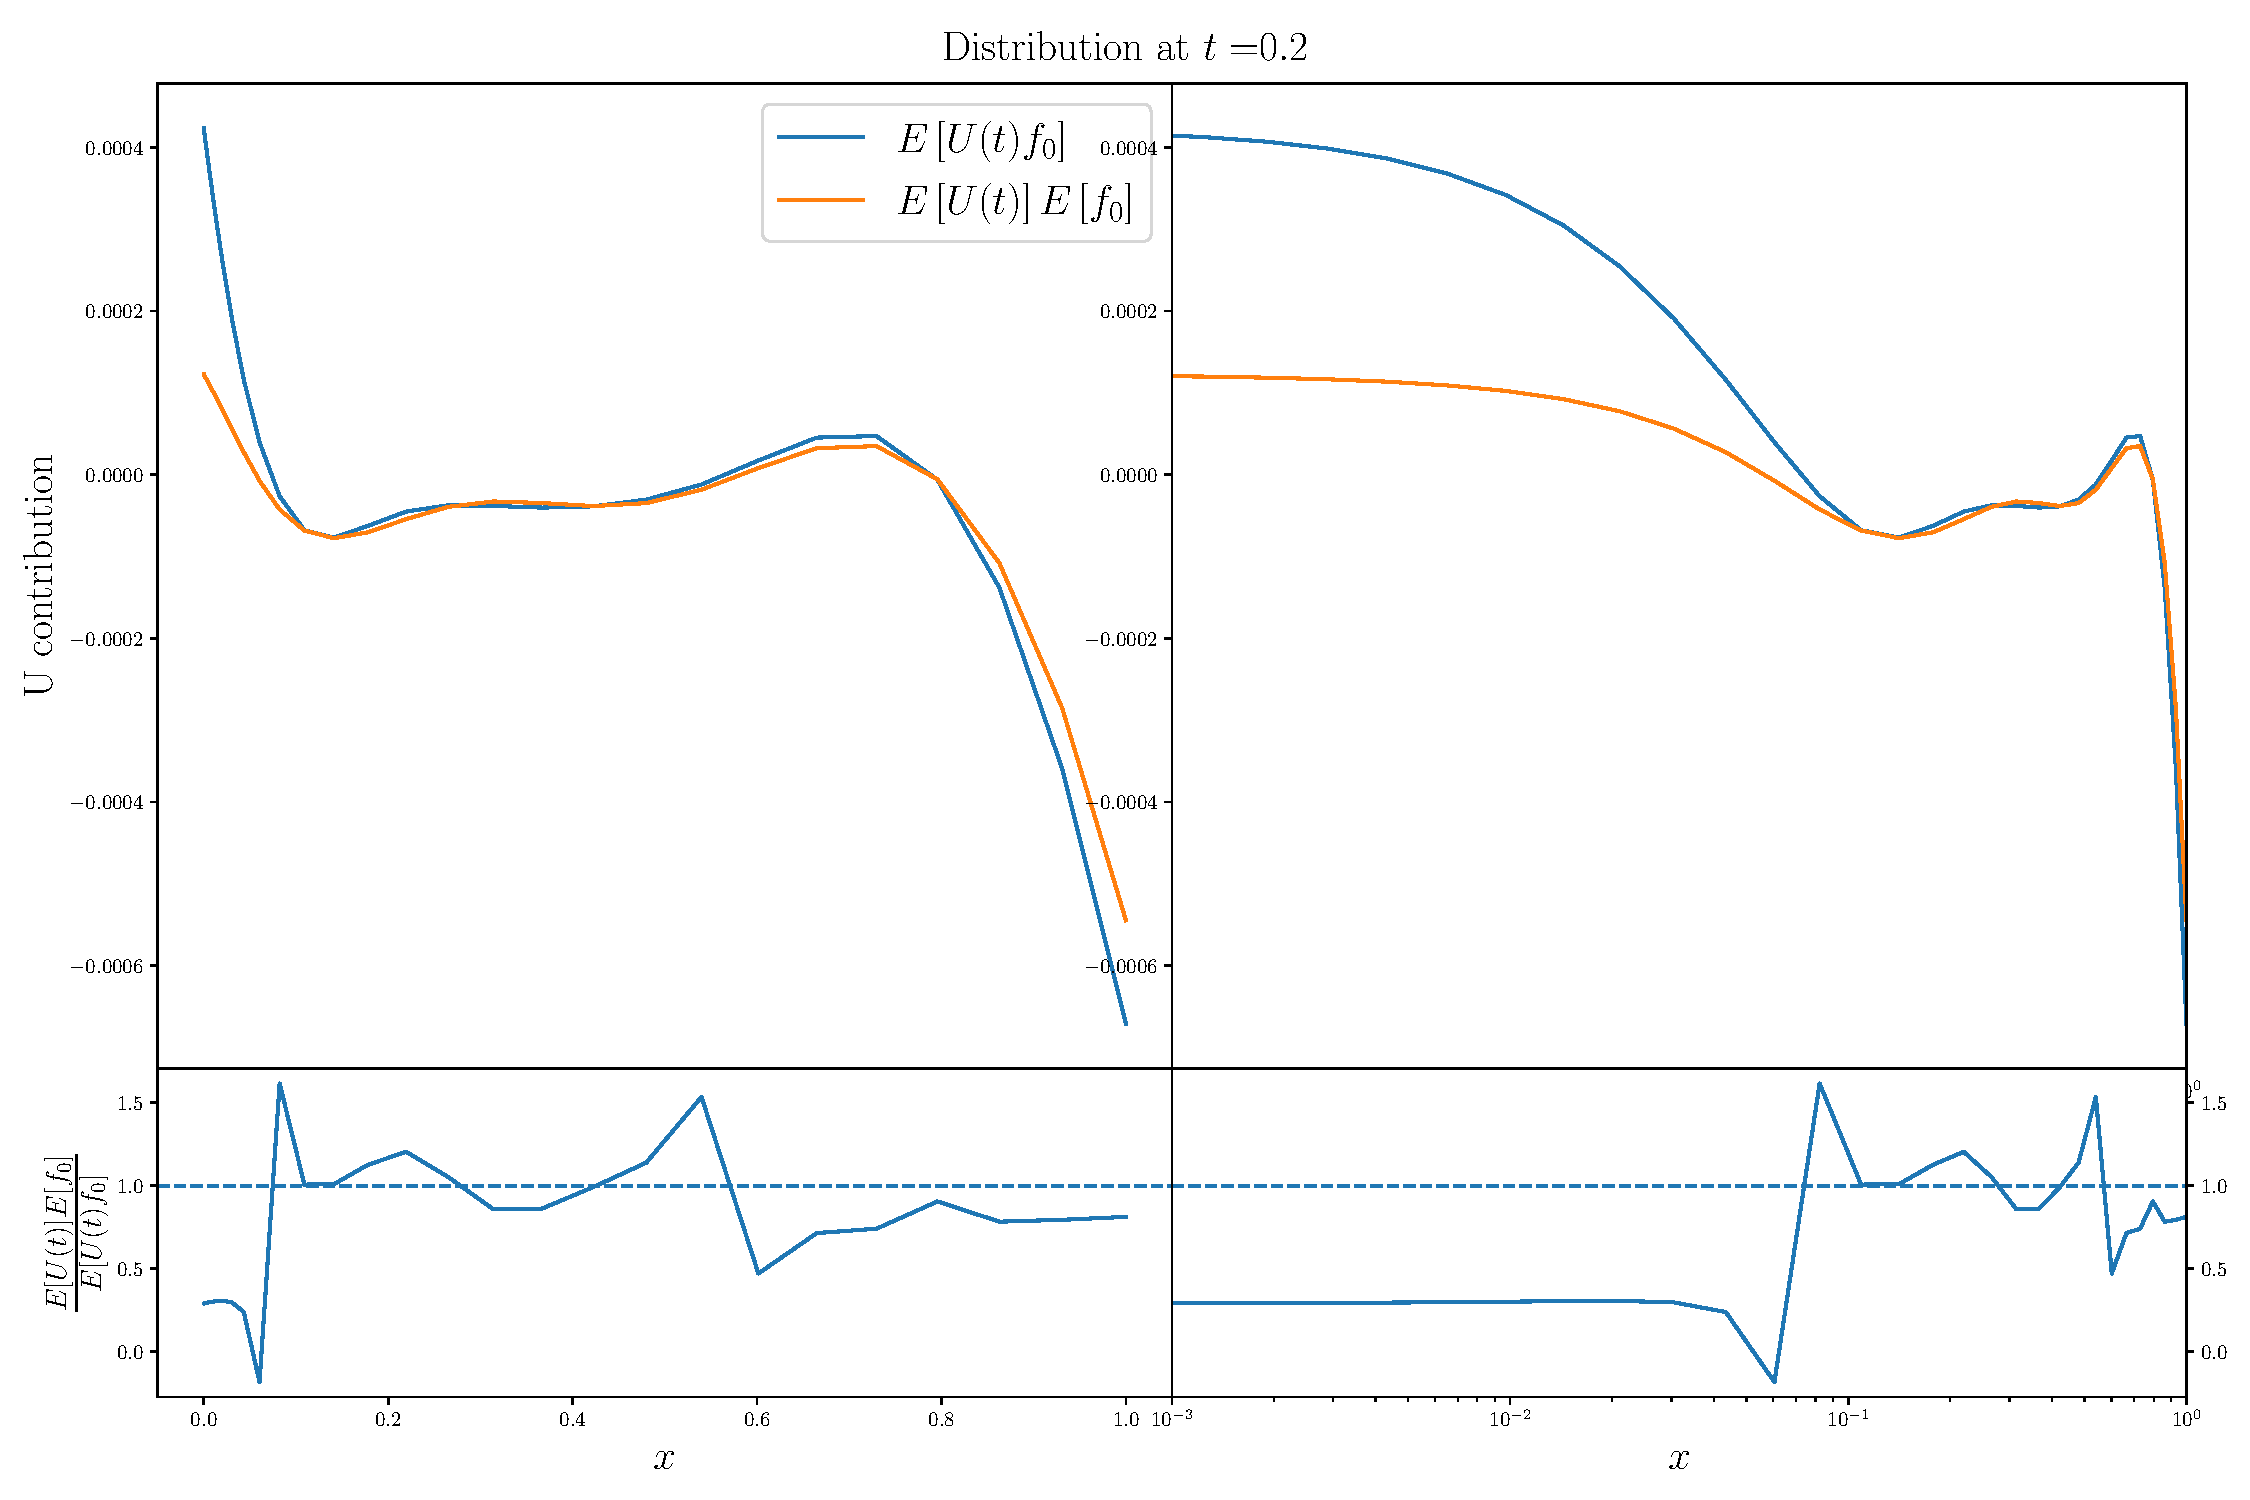
\includegraphics[width=0.65\textwidth]{plots/xT3_exp_val_eot.pdf}
  \caption{Expectation value of the product (blue) and product of the expectation value
  for the $U$ contribution. Plots obtained using $t_{\rm ref} = 30000$, while $f_0$ is
  an ensemble of networks at initialisation (\textit{i.e.} $\mathbb{E}[f_0]=0$).
  \ac{These plots will be modified (font size, etc...) to match the other figures.}}
\end{figure}
% ===================================
